%
% chapter.tex -- Kapitel 2: Koordinaten und Tangentialvektoren
%
% (c) 2024 Prof Dr Andreas Müller
%
\chapter{Koordinaten und Tangentialvektoren
\label{chapter:koordinaten}}
Die Bühne der Physik ist ein Raum von Punkten, in dem wir geometrische
Konstruktionen anwenden und zum Beispiel Bahnen von Körpern beschreiben
können.
Solche Beschreibungen verwenden immer mehr oder weniger speziell gewählte
Koordinatensysteme, die Punkte durch Koordinaten beschreiben.
Da die Koordinaten nur ein Werkzeug zur physikalischer Gegebenheiten
sind, muss es immer möglich sein, die zur Formulierung von Naturgesetzen
entwickelten Abstraktionen wie Kurven, Funktionen oder Vektoren zwischen
beliebigen Koordinatensystemen umzurechnen.
Ziel dieses Kapitels ist daher, eine für alle Arten von Koordinatensystemen
nützliche Notation zu entwickeln, die Umrechnung zwischen Koordinatensystemn
zu studieren und den Begriff des Tangentialvektors einzuführen.

%
% Koordinaten
%
\section{Koordinaten
\label{buch:koordinaten:section:koordinaten}}
In diesem Abschnitt betrachten wir eine Punktemeng $X$, die mit
Koordinatensystemen ausgestattet werden soll.

\subsection{Koordinatensystem}
Ein $n$-dimensionales Koordinatensystem auf $X$ ordnet jedem Punkt 
ein $n$-Tupel von Koordinaten zu.
Aus erst später verständlichen Gründen bezeichnen wir die Koordinaten
mit hochgestellten Indizes, wir schreiben also $x^1,\dots,x^n$.
Eine Verwechslungsgefahr mit Exponenten besteht normalerweise nicht.
Falls die $k$-te Potenz der Koordinate $x^1$ berechnet werden soll, 
wird dies mit Klammern als $(x^i)^k$ geschrieben.
Ein Koordinatensystem ist also eine Abbildung
\[
\varphi
\colon
X\to \mathbb{R}^n
:
x \mapsto (x^1,\dots,x^n).
\]

\begin{beispiel}
\label{buch:koordinaten:koordinaten:beispiel:kartpolar}
%
% fit-kartpolar.tex%
%
% (c) 2024 Prof Dr Andreas Müller
%
\begin{figure}
\centering
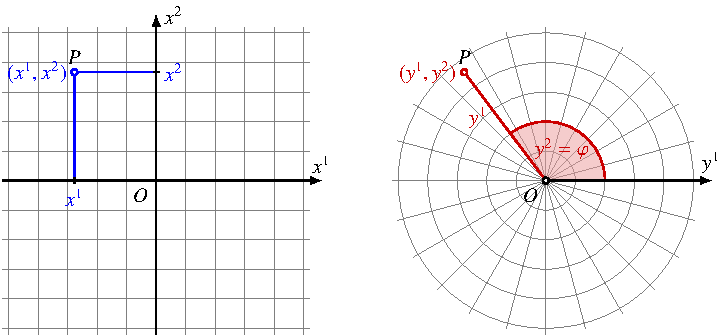
\includegraphics{chapters/020-koordinaten/images/kartpolar.pdf}
\caption{Zwei Koordinatensysteme für die Ebene:
kartesische (rechtwinklige) Koordinaten links und Polarkoordinaten
rechts.
Der gleiche Punkt $P$ wird gleichermassen durch die Koordinaten 
$(x^1,x^2)$ und $(y^1,y^2)$ beschrieben.
\label{buch:koordinaten:fig:kartpolar}}
\end{figure}

Die Punkte einer Ebene können einerseits mit dem {\em kartesischen}
Koordinatensystem mit den Koordinaten $(x^1,x^2)\in\mathbb{R}$ 
beschrieben werden und andererseits durch {\em Polarkoordinaten},
\index{Polarkoordinaten}%
die einen Punkt durch den Radius $y^1 = r$ und den Polarwinkel
$y^2 = \varphi$ definieren (Abbildung~\ref{buch:koordinaten:fig:kartpolar}).

Die kartesischen Koordinaten können aus den Polarkoordinaten durch
\begin{equation}
\left.
\begin{aligned}
x^1 &= y^1\cos y^2 \\
x^2 &= y^1\sin y^2
\end{aligned}
\qquad
\right\}
\label{buch:koordinaten:koordinaten:eqn:polarkartumrechnung}
\end{equation}
berechnet werden.
\end{beispiel}

\begin{beispiel}
\label{buch:koordinaten:koordinaten:beispiel:kartkugel}
%
% fig-kartkugel.tex
%
% (c) 2024 Prof Dr Andreas Müller
%
\begin{figure}
\centering
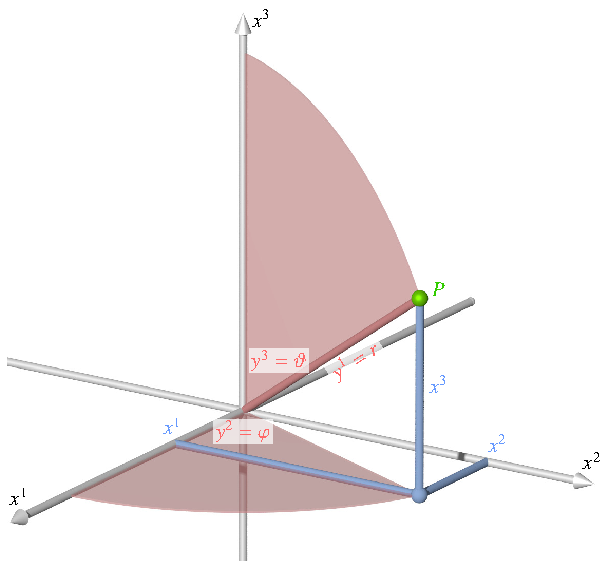
\includegraphics{chapters/020-koordinaten/images/kartkugel.pdf}
\caption{Kartesische Koordinaten ({\color{blue}blau}) und Kugelkoordinaten
({\color{darkred}rot}) für einen Punkt $P$ des dreidmensionalen Raumes.
\label{buch:koordinaten:koordinaten:fig:kartkugel}}
\end{figure}

Der dreidimensionale Raum kann sowohl durch {\em kartesische}
Koordinatentripel $(x^1,x^2,x^3)$ wie auch durch {\em Kugelkoordinaten}
\index{Kugelkoordinaten}%
beschrieben werden.
In Kugelkoordinaten ist ein Punkt durch die Entfernung $r=y^1$ vom
Nullpunkt, den Polarwinkel $y^2=\varphi$ seiner Projektion in die 
$x^1$-$x^2$-Ebene und den Winkel $\vartheta$ zwischen der positiven
$x^3$-Achse und der Geraden durch Nullpunkt $O$ und den Punkt gegeben
(Abbildung~\ref{buch:koordinaten:koordinaten:fig:kartkugel}).
Die Umrechnung von Kugelkoordinaten in kartesische Koordinaten
erfolgt mit
\begin{equation}
\left.
\begin{aligned}
x^1
&=
y^1 \cos y^2 \cos y^3 \\
x^2
&=
y^1 \sin y^2 \cos y^3 \\
x^3
&=
y^2 \cos y^3.
\end{aligned}
\qquad\right\}
\label{buch:koordinaten:koordinaten:eqn:kugelkartumrechnung}
\end{equation}
Man beachte, dass Punkte auf der $x^3$-Achse $y^3=0$ oder
$y^3=\pi$ und beliebigen Winkel $y^2\in\mathbb{R}$ haben.
Ohne zusätzliche Einschränkungen haben die Punkte auf der
$x^3$-Achse keine eindeutigen Kugelkoordinaten.
\end{beispiel}

% XXX Abbildung: Koordinatenabbildung

Auf der Menge $X$ sind bis jetzt keinerlei weitere Eigenschaften definiert,
welche anzeigen können, ob Punkte nahe beeinander sind, wie man das zum
Beispiel bei der Formulierung von Grenzwerten oder Ableitungen braucht.
Diese Eigenschaften können aber mithilfe der Koordinatenabbildung
gewonnen werden.
Dazu müssen aber die Koordinatenabbildungen weiter eingeschränkt
werden.
Zunächst muss die Koordinatenabbildung bijektiv sein.
Dies bedeutet, dass jeder Punkt durch genau ein Koordinaten-$n$-Tupel
beschrieben wird.
Ausserdem muss die Menge $U$ der möglichen Koordinaten-$n$-Tupel eine
offene Menge in $\mathbb{R}^n$ sein.

% XXX Beispiel zur Notwendigkeit der letzten Bedingung zeigen

\subsection{Koordinatenwechsel}
In den Beispielen
\ref{buch:koordinaten:koordinaten:beispiel:kartpolar}
und
\ref{buch:koordinaten:koordinaten:beispiel:kartkugel}
wurden bereits Umrechnungsformeln zwischen den dort dargestellten
Koordinatensystemen ermittelt.
Seien etwas allgemeiner zwei Koordinatensysteme $x^1,\dots,x^n$
und $y^1,\dots,y^n$ auf der Punktmenge $X$ gegeben.
Wenn $U$ die Menge der Koordinaten-$n$-Tupel ist, die Punkte von $X$
in den $x^i$-Koordinaten beschreiben, dann ist die Koordinatenumrechnung
vom $x^i$-Koordinatensystem in das $y^i$-Koordinatensystem eine Abbildung
\[
\varphi
\colon
U\to\mathbb{R}^n
:
(x^1,\dots,x^n)
\mapsto
(y^1,\dots,y^n)
\]
von $U$ in $\mathbb{R}^n$.


\subsubsection{Stetigkeit}

\subsubsection{Differenzierbarkeit}

\subsubsection{Topologische Räume}

%
% Tangentialvektoren
%
\section{Tangentialvektoren
\label{buch:koordinaten:section:tangentialvektoren}}

%
% Differentialoperatoren
%
\section{Differentialoperatoren
\label{buch:koordinaten:section:differentialoperatoren}}

%
% Differenzierbare Atlanten und differenzierbare Mannigkfaltigkeiten
%
\section{Differenzierbare Mannigfaltigkeiten
\label{buch:koordinatne:section:mannigfaltigkeiten}}



